\chapter{System Design}

This chapter describes the architecture and design decisions behind \textit{TRiM}. It covers the overall system structure, multi-tenant data isolation strategy, core business logic, frontend design, and deployment set up.

\section{System Overview}
\textit{TRiM} is built as a multi-tenant Software-as-a-Service (SaaS) platform following a three-tier architecture: a React single-page application on the frontend, a Spring Boot REST API on the backend, and a PostgreSQL database for persistence. Each tenant (i.e. each business using the platform) is identified by a unique subdomain such as \texttt{v7.trimbooking.ie}, and all three tiers are tenant-aware, which means every request is scoped to a single business from the moment it enters the system.

The frontend is a TypeScript React app bundled with Vite and served by Nginx. It communicates with the backend through a RESTful JSON API. The backend is a stateless Spring Boot application that handles authentication, business logic, and data access. Authentication is token-based using JSON Web Tokens (JWT), with no server-side session state. As discussed earlier, PostgreSQL was selected specifically for its native support for RLS, which enforces tenant isolation at the database level and ensures that even a bug in application code cannot expose businesses' data.

Integrations include Stripe Connect for payment processing, where each business connects their own Stripe account to receive deposits directly, and Twilio and SMTP for sending booking confirmation notifications via SMS and email.

The system is containerised using Docker Compose, with three services: the PostgreSQL database, the Spring Boot API, and the Nginx-served frontend. In production, all three containers run on a Virtual Private Server (VPS), an Infrastructure-as-a-Service (IaaS) deployment, with Nginx acting as a reverse proxy.

\subsection*{Architecture Diagram}
Figure~\ref{fig:architecture} illustrates the high-level architecture of the system, showing the request flow from the browser through Nginx and the Spring Boot filter chain to PostgreSQL, along with the external service integrations.

\begin{figure}[H]
    \centering
    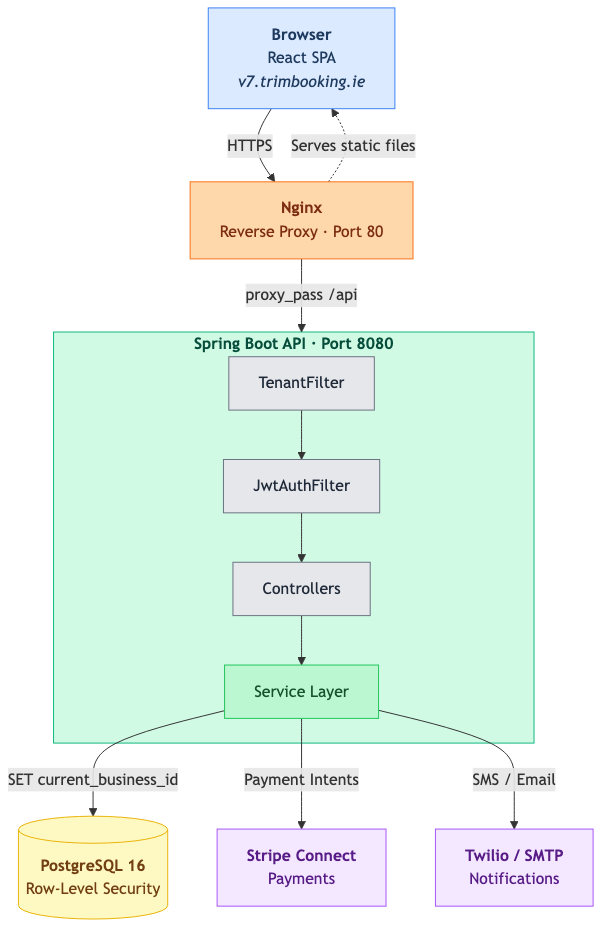
\includegraphics[width=0.6\textwidth]{images/architecture.png}
    \caption{High-level system architecture diagram.}
    \label{fig:architecture}
\end{figure}

\subsection*{RESTful API Design}
The backend exposes a RESTful JSON API under the \texttt{/api} prefix. All endpoints follow standard REST conventions: resources are identified by URL paths, operations map to HTTP methods (GET, POST, DELETE, etc.), and all request and response bodies use JSON. The API is entirely stateless and there are no server-side sessions. Every authenticated request requires a JWT passed in the \texttt{Authorization} header.

Endpoints are split into two categories. Public endpoints, such as login, registration, active service listings, availability lookups, and the Stripe webhook, can be accessed without authentication. All remaining endpoints require a valid JWT, and Spring Security rejects any request that does not carry one. Because the system is multi-tenant, every request also carries the business context implicitly through the subdomain or \texttt{X-Business-Slug} header. No endpoint requires a \texttt{businessId} parameter. The \texttt{TenantFilter} resolves it automatically before the request reaches any controller.

Listing~\ref{lst:axios-interceptor} shows the Axios request interceptor on the frontend, which attaches both the JWT and the business slug header to every outgoing API call.

\begin{lstlisting}[caption={Axios request interceptor attaching JWT and tenant context to every API call.}, label={lst:axios-interceptor}]
// Request interceptor - Add JWT token and business slug to every request
api.interceptors.request.use(
  (config) => {
    const token = localStorage.getItem("token");
    if (token) {
      config.headers.Authorization = `Bearer ${token}`;
    }

    // Send business slug header only when present
    const businessSlug = getBusinessSlug();
    if (businessSlug) {
      config.headers["X-Business-Slug"] = businessSlug;
    }

    return config;
  },
  (error) => {
    return Promise.reject(error);
  },
);
\end{lstlisting}

Table~\ref{tab:api-endpoints} summarises the main API endpoint groups exposed by the Java backend.

\begin{table}[H]
    \centering
    \begin{tabularx}{\textwidth}{|l|l|X|}
    \hline
    \textbf{Resource} & \textbf{Prefix} & \textbf{Description} \\
    \hline
    Authentication & \texttt{/api/auth} & Login, register, password reset, cross-subdomain token exchange \\
    \hline
    Bookings & \texttt{/api/bookings} & Create, reschedule, cancel, mark complete or no-show \\
    \hline
    Barbers & \texttt{/api/barbers} & Create, update, activate and deactivate barber profiles \\
    \hline
    Barber Breaks & \texttt{/api/barber-breaks} & Manage scheduled break times per barber \\
    \hline
    Availability & \texttt{/api/availability} & Query available time slots for a given barber, date, and service \\
    \hline
    Barber Availability & \texttt{/api/barber-availability} & Set and update weekly working hours per barber \\
    \hline
    Services & \texttt{/api/services} & Create, update, and deactivate services offered \\
    \hline
    Categories & \texttt{/api/categories} & Manage service categories with nested service listings \\
    \hline
    Payments & \texttt{/api/payments} & Create Stripe payment intents and handle webhooks \\
    \hline
    Stripe Connect & \texttt{/api/stripe-connect} & Business onboarding, account status, dashboard access \\
    \hline
    Customers & \texttt{/api/admin/customers} & List customers, blacklist and unblacklist \\
    \hline
    Dashboard & \texttt{/api/dashboard} & Admin statistics and revenue metrics \\
    \hline
    \end{tabularx}
    \caption{Summary of API endpoint groups.}
    \label{tab:api-endpoints}
\end{table}

\section{Multi-Tenant Database Design}
This section describes the multi-tenant data isolation strategy used in \textit{TRiM}, which is a critical aspect of the system's design. The main goal is to ensure that each tenant's data is completely isolated and secure, while still allowing for efficient querying and scalability.

\subsection*{Entity-Relationship Model}
\begin{figure}[H]
    \centering
    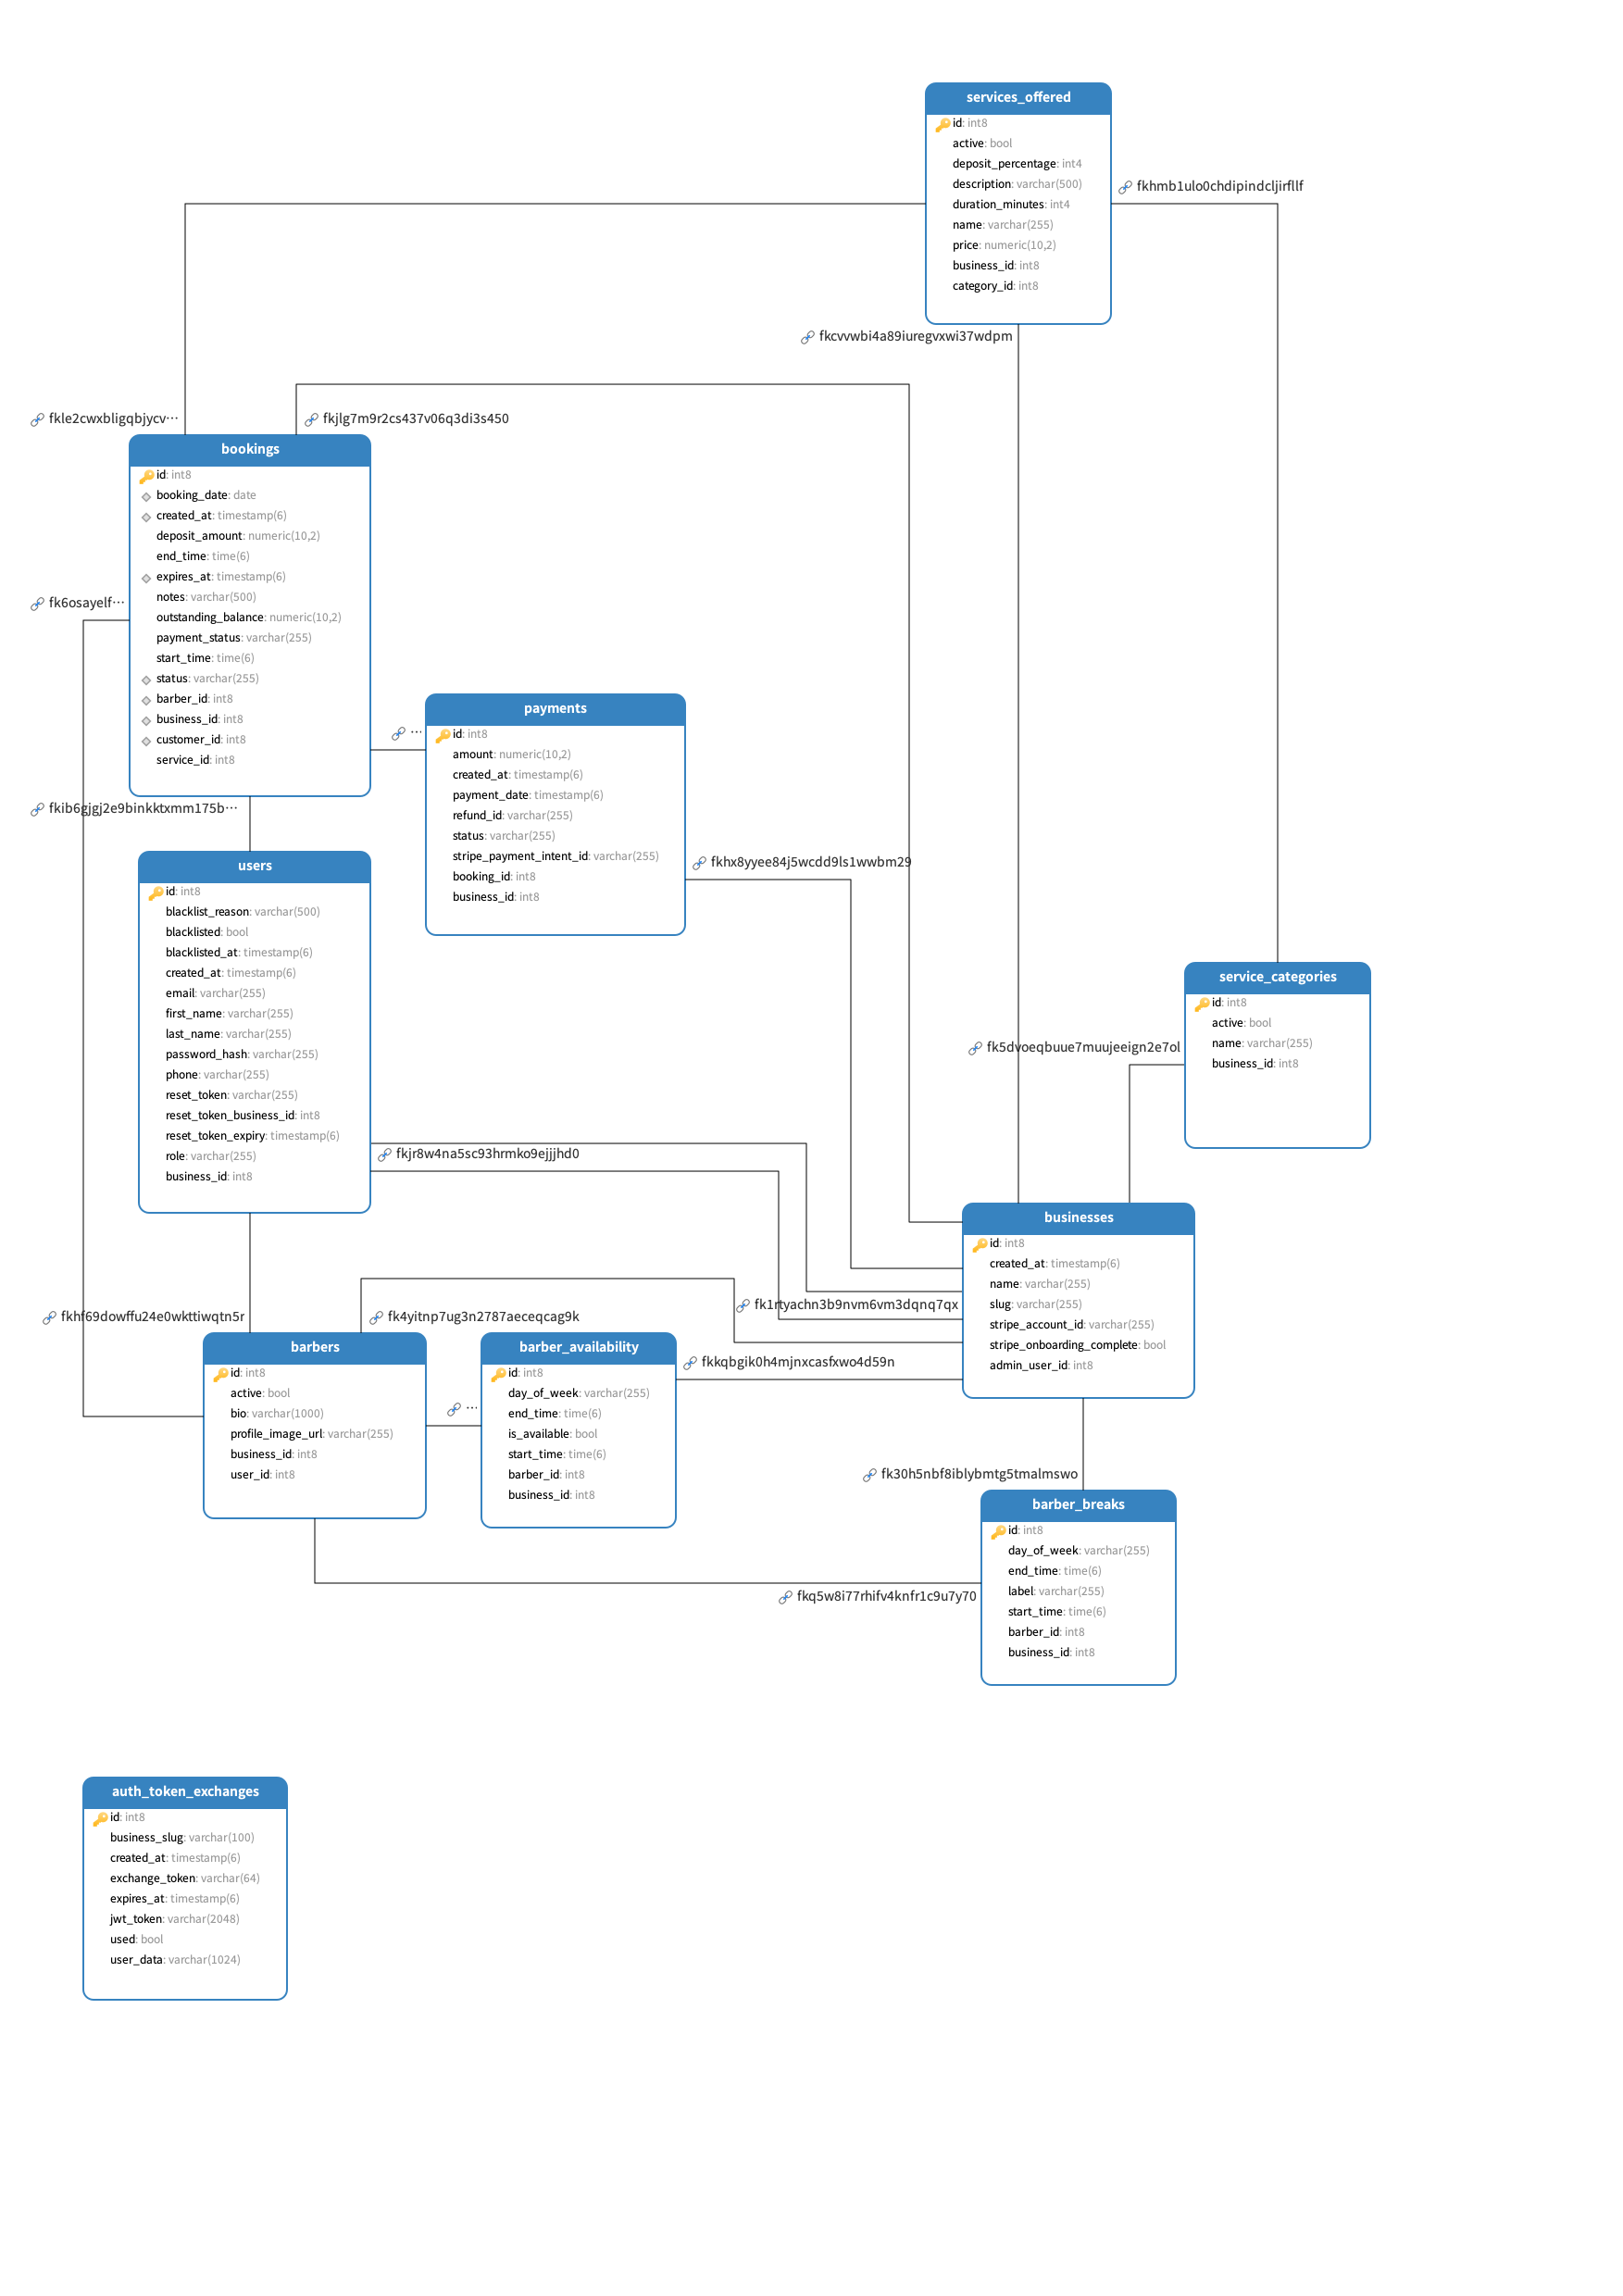
\includegraphics[width=0.9\textwidth]{images/db.png}
    \caption{Entity-Relationship diagram of the PostgreSQL database schema.}
    \label{fig:er-diagram}
\end{figure}

Figure~\ref{fig:er-diagram} shows the full database schema. The central entity is \texttt{businesses}, which represents a tenant. Nearly every other table carries a \texttt{business\_id} foreign key that ties its rows to a specific business, forming the foundation of the multi-tenant isolation model.

The core domain relationships are as follows. A \texttt{booking} links a customer (\texttt{users}), a \texttt{barber}, and a \texttt{service\_offered}, along with the date, time slot, and status. Each booking may have an associated \texttt{payment} record that tracks the Stripe payment intent and deposit amount. Barbers have two supporting tables: \texttt{barber\_availability} defines their weekly working hours, and \texttt{barber\_breaks} defines scheduled breaks within those hours. Services are grouped into \texttt{service\_\allowbreak categories}, with each service belonging to one category.

The \texttt{users} table stores all user types (customers, barbers, and admins) distinguished by a \texttt{role} column. Barbers are linked to their user account via a \texttt{user\_id} foreign key, while the business's admin is referenced by \texttt{admin\_user\_id} on the \texttt{businesses} table.

The only table without a \texttt{business\_id} is \texttt{auth\_token\_exchanges}, which stores short-lived tokens used for cross-subdomain authentication. These tokens operate across tenants by design, as they facilitate the redirect from the main registration page to a tenant-specific subdomain.

\subsection*{Migrating From Single to Multi-Tenant}
The system was initially developed as a single-tenant application, with all entities (users, barbers, bookings, services) existing in a single flat schema with no concept of business ownership. Once the core functionality was done, the codebase was refactored to support multiple tenants. This involved some key changes:

\begin{itemize}
    \item A new \texttt{businesses} table was introduced to represent each tenant, with a unique \texttt{slug} used for subdomain-based identification.
    \item A \texttt{business\_id} foreign key column was added to every tenant-scoped table, linking each row to its owning business.
    \item JPA entity classes were updated to include a \texttt{@ManyToOne} relationship to \texttt{Business}, and repository queries were updated to filter by \texttt{business\_id}.
    \item The JWT token payload was extended to include a \texttt{businessId} claim, so that each token is bound to a specific tenant.
    \item A request filter chain was introduced (\texttt{TenantFilter} and \texttt{JwtAuthenticationFilter}) to resolve and validate the tenant context on every request, as described later in this chapter.
    \item PostgreSQL Row-Level Security policies were applied to enforce isolation at the database level, independent of application code.
\end{itemize}

This incremental approach meant that the single-tenant version served as a working prototype, and the multi-tenant refactor could be layered on top without redesigning the core logic.

\section{Multi-Tenant Implementation}
A common approach to multi-tenant isolation is to filter data purely in application code, for example by appending \texttt{WHERE business\_id = ?} to every query. While straightforward, this approach is fragile: a single forgotten filter or a new repository method without a tenant check is enough to leak data across businesses.

As identified in the literature review (Chapter~3), PostgreSQL Row-Level Security (RLS) offers a stronger alternative. RLS policies are defined at the database level and automatically filter every \texttt{SELECT}, \texttt{INSERT}, \texttt{UPDATE}, and \texttt{DELETE} operation based on a session variable. The application cannot bypass these policies, regardless of how the query is constructed.

\textit{TRiM} uses both approaches together as a defence-in-depth strategy, summarised in Table~\ref{tab:isolation-layers}. Any single layer is sufficient to prevent cross-tenant data access; together they ensure that even if one layer fails, the others still enforce isolation. The remainder of this section describes how each layer is implemented.

\begin{table}[H]
    \centering
    \begin{tabular}{|p{0.20\textwidth}|p{0.35\textwidth}|p{0.4\textwidth}|}
    \hline
    \textbf{Layer} & \textbf{Mechanism} & \textbf{What it prevents} \\
    \hline
    Application & Repository methods filter by \texttt{business\_id} & Queries are scoped to the current tenant by design \\
    \hline
    Authentication & JWT \texttt{businessId} must match \texttt{TenantContext} & Tokens issued for one business cannot be used on another \\
    \hline
    Database & PostgreSQL RLS policies & Even if both application layers fail, the database will not return rows outside the current tenant \\
    \hline
    \end{tabular}
    \caption{Three independent layers of tenant data isolation.}
    \label{tab:isolation-layers}
\end{table}

\subsection*{How Is a Request Scoped to a Tenant?}
Every incoming request must be associated with a specific business before any controller logic runs. This is handled by two components working together: \texttt{TenantContext}, a thread-local store, and \texttt{TenantFilter}, a request filter.

\texttt{TenantContext} is a utility class that uses Java's \texttt{ThreadLocal} to hold the current business ID and slug for the duration of a single HTTP request. It is written to by the \texttt{TenantFilter} at the start of the request, read by the \texttt{RlsDataSource} when a database connection is checked out, and cleared in a \texttt{finally} block to prevent memory leaks.

\texttt{TenantFilter} is a request filter that runs before the JWT authentication filter in the security filter chain. It resolves which business the request is for using three strategies, in this order:

\begin{enumerate}
    \item \textbf{Subdomain} -- the first part of the hostname is extracted (e.g. \texttt{v7.trimbooking.ie} yields \texttt{v7}). Common subdomains such as \texttt{www}, \texttt{api}, and \texttt{localhost} are ignored.
    \item \textbf{Header} -- the \texttt{X-Business-Slug} header, sent by the frontend's Axios interceptor on every request.
    \item \textbf{Query parameter} -- a \texttt{?business=slug} fallback for development and testing.
\end{enumerate}

Once a slug is resolved, the filter looks up the \texttt{Business} entity by slug. If found, it calls \texttt{TenantContext.setCurrentBusiness()} and the request proceeds. If no slug is provided or the business does not exist, the request is rejected with a 400 or 404 response before it reaches any controller.

Certain endpoints are exempted from tenant resolution because they operate outside the scope of a single business such as admin registration (which creates a new business), the cross-subdomain token exchange endpoint, and the Stripe payment webhook.

Listing~\ref{lst:tenant-filter} shows the core of the filter's resolution logic.

\begin{lstlisting}[caption={TenantFilter extracting business slug from multiple sources.}, label={lst:tenant-filter}]
private String extractBusinessSlug(HttpServletRequest request) {
    // Strategy 1: Extract from subdomain
    String slug = extractFromSubdomain(request);
    if (slug != null && !slug.isEmpty()) return slug;

    // Strategy 2: X-Business-Slug header
    slug = request.getHeader("X-Business-Slug");
    if (slug != null && !slug.isEmpty()) return slug;

    // Strategy 3: Query parameter
    slug = request.getParameter("business");
    if (slug != null && !slug.isEmpty()) return slug;

    return null;
}
\end{lstlisting}

\subsection*{Cross-Subdomain Token Exchange}
When a new admin registers on the main site, the system creates their business and issues a JWT token. The user then needs to be redirected to their tenant-specific subdomain (e.g. \texttt{v7.trimbooking.ie}). However, the JWT cannot simply be passed along: cookies do not transfer across subdomains, and placing a long-lived token in a URL query parameter would be insecure as it could be leaked through browser history or server logs.

To solve this, \textit{TRiM} uses a short-lived, single-use exchange token. The flow works as follows:

\begin{enumerate}
    \item After registration, the backend generates a cryptographically secure random token (32 bytes, Base64 URL-encoded) and stores it in the \texttt{auth\_token\_\allowbreak exchanges} table alongside the actual JWT, the user data, and the target business slug. The exchange token expires after 60 seconds.
    \item The user is redirected to the target subdomain with the exchange token in the URL (e.g. \texttt{v7.trimbooking.ie/auth?token=abc123}).
    \item The frontend on the target subdomain sends the exchange token to the \texttt{/api/auth/exchange-token} endpoint, which looks up the token, validates that it has not expired or been used, marks it as used, and returns the actual JWT and user data.
    \item The frontend stores the JWT in \texttt{localStorage} and the user is authenticated on the new subdomain.
\end{enumerate}

This approach ensures that the actual JWT is never exposed in a URL. The exchange token is single-use, short-lived, and cryptographically random, making it safe to pass as a query parameter. A scheduled task cleans up expired and used tokens every five minutes.

\section{Business Operations}
This section describes the core business logic of the platform: how a customer books an appointment, how deposits are collected through Stripe, and how the system prevents two customers from booking the same time slot simultaneously.

\subsection*{Booking \& Payment Flow}
The booking and payment process in \textit{TRiM} follows a three-phase flow: the customer creates a booking, pays a deposit through Stripe, and the system confirms the booking once payment succeeds. Each phase is described below.

\subsubsection*{Phase 1: Booking Creation}
When a customer submits a booking request, the backend runs through a series of validation and conflict-detection steps inside the database transaction:

\begin{enumerate}
    \item \textbf{Entity validation}: the customer, barber, and service are loaded from the database and verified to exist and belong to the same business.
    \item \textbf{Blacklist check}: if the customer has been blacklisted by the business, the request is rejected.
    \item \textbf{Time validation}: the requested date and time must be in the future.
    \item \textbf{Conflict detection}: the system acquires a pessimistic lock on all existing bookings for that barber and date, then checks for time overlaps. This step is described in the next subsection.
    \item \textbf{Booking saved}: if no conflicts are found, the booking is persisted with a status of \texttt{PENDING} and an expiry time set to ten minutes from now.
\end{enumerate}

The ten-minute expiry is intentional. A pending booking holds a time slot, preventing other customers from booking it. If, for some reason, the payment is not completed within ten minutes, the booking expires and the slot is released. Expired bookings are excluded from conflict detection and are periodically cleaned up by a scheduled task that marks them as \texttt{CANCELLED}.

\subsubsection*{Phase 2: Deposit Payment via Stripe}
After the booking is created, the frontend calls \texttt{/api/payments/create-intent} to initiate the deposit payment. The backend calculates the deposit as a percentage of the service price (configured per service and set by the ADMIN user), verifies that the business has completed Stripe Connect onboarding, and creates a Stripe \texttt{PaymentIntent} on the business's connected account. The key point is that \textit{TRiM} uses Stripe Connect in its Standard model: each business connects their own Stripe account during onboarding, and deposits are paid directly into that account. The platform does not hold customer funds.

The \texttt{PaymentIntent} includes the \texttt{booking\_id} and \texttt{business\_id} in its metadata, which are used later for webhook verification. The backend returns the Stripe \texttt{clientSecret} to the frontend, which renders the Stripe payment form using Stripe Elements. The customer completes the payment (card, Apple Pay, or Google Pay) entirely on the client side.

\subsubsection*{Phase 3: Webhook Confirmation}
Once Stripe processes the payment, it sends a \texttt{payment\_intent.succeeded} event to the \texttt{/api/payments/webhook} endpoint. The webhook handler performs several verification steps before confirming the booking:

\begin{enumerate}
    \item \textbf{Signature verification}: the \texttt{Stripe-Signature} header is validated against the webhook secret to ensure the request genuinely came from Stripe.
    \item \textbf{Cross-tenant verification}: the \texttt{business\_id} from the payment metadata is compared against the booking's actual business, and the Stripe connected account ID on the event is compared against the business's stored account ID. A mismatch in either check rejects the webhook.
    \item \textbf{Booking confirmation}: the payment record is marked as \texttt{SUCCEEDED}, the booking status transitions from \texttt{PENDING} to \texttt{CONFIRMED}, the deposit amount is recorded, and the ten-minute expiry is cleared.
    \item \textbf{Notifications}: a confirmation email and SMS are sent to the customer with the booking details.
\end{enumerate}

Listing~\ref{lst:webhook-handler} shows the \texttt{handlePaymentSuccess} method that executes steps 2--4. Because the webhook originates from Stripe rather than from a tenant-scoped browser request, the method manually sets the RLS context using the business ID from the payment metadata before performing any database queries.

\begin{lstlisting}[caption={Webhook handler confirming a booking after successful deposit payment.}, label={lst:webhook-handler}]
@Transactional
public void handlePaymentSuccess(String paymentIntentId,
                                  Long businessIdFromMetadata) {
    // Set RLS context manually (webhook has no tenant filter)
    entityManager.createNativeQuery(
        "SELECT set_config('app.current_business_id', ?1, true)")
        .setParameter(1, String.valueOf(businessIdFromMetadata))
        .getSingleResult();

    Payment payment = paymentRepository
        .findByStripePaymentIntentId(paymentIntentId)
        .orElseThrow(() -> new RuntimeException("Payment not found"));

    Booking booking = payment.getBooking();

    // Verify business_id from metadata matches booking's business
    if (!businessIdFromMetadata.equals(booking.getBusiness().getId())) {
        throw new RuntimeException(
            "Payment business verification failed");
    }

    // Update payment and booking status
    payment.setStatus(Payment.PaymentStatus.SUCCEEDED);
    payment.setPaymentDate(LocalDateTime.now());
    paymentRepository.save(payment);

    booking.setPaymentStatus(Booking.PaymentStatus.DEPOSIT_PAID);
    booking.setStatus(Booking.BookingStatus.CONFIRMED);
    booking.setExpiresAt(null);
    bookingRepository.save(booking);

    // Send confirmation notifications
    emailService.sendBookingConfirmation(booking);
    smsService.sendBookingConfirmation(booking);
}
\end{lstlisting}

\subsection*{Race Condition Prevention When Booking}
A race condition occurs when two or more concurrent requests read the same state and both act on it before either write is committed. In a booking system, this means two customers could simultaneously check availability for the same barber at the same time slot, both see it as free, and both successfully create a booking, resulting in a double-booking. This is known as a time-of-check-to-time-of-use (TOCTOU) problem.

\textit{TRiM} prevents this using pessimistic locking at the database level. When a booking is being created, the conflict detection query acquires an exclusive write lock on all existing booking rows for that barber and date. This is done using JPA's \texttt{@Lock} annotation, which translates to a PostgreSQL \texttt{SELECT ... FOR UPDATE} statement. While one transaction holds this lock, any other transaction attempting to book the same barber on the same date will block until the first transaction either commits or rolls back. This serialises concurrent booking attempts and eliminates the race condition entirely.

Listing~\ref{lst:pessimistic-lock} shows the repository method that acquires the lock.

\begin{lstlisting}[caption={Pessimistic write lock on booking rows for conflict detection.}, label={lst:pessimistic-lock}]
@Lock(LockModeType.PESSIMISTIC_WRITE)
@Query("SELECT b FROM Booking b " +
       "WHERE b.business.id = :businessId " +
       "AND b.barber.id = :barberId " +
       "AND b.bookingDate = :bookingDate")
List<Booking> findByBusinessIdAndBarberIdAndBookingDateWithLock(
    @Param("businessId") Long businessId,
    @Param("barberId") Long barberId,
    @Param("bookingDate") LocalDate bookingDate);
\end{lstlisting}

Once the rows are locked and returned, the \texttt{BookingConflictDetectionService} iterates over them and checks for time overlaps. Cancelled bookings and expired pending bookings are skipped, since those slots are available for reuse. The overlap check uses a standard interval comparison: two time slots overlap if and only if the first starts before the second ends and the first ends after the second starts.

Listing~\ref{lst:conflict-detection} shows the conflict detection logic.

\begin{lstlisting}[caption={Time slot conflict detection with pessimistic locking.}, label={lst:conflict-detection}]
public void validateTimeSlotAvailable(Long barberId,
        LocalDate bookingDate, LocalTime startTime, LocalTime endTime) {
    List<Booking> existingBookings = bookingRepository
        .findByBusinessIdAndBarberIdAndBookingDateWithLock(
            getBusinessId(), barberId, bookingDate);

    for (Booking existing : existingBookings) {
        if (existing.getStatus() == BookingStatus.CANCELLED) continue;
        if (existing.isExpired()) continue;

        // Overlap: start1 < end2 AND end1 > start2
        if (startTime.isBefore(existing.getEndTime())
                && endTime.isAfter(existing.getStartTime())) {
            throw new ConflictException(
                "This time slot is no longer available");
        }
    }
}
\end{lstlisting}

It is worth noting that the availability endpoint used by the frontend to display open slots does \textit{not} acquire a lock, it performs a regular read query. This is intentional: locking during availability checks would degrade performance for a read-heavy operation that does not modify data. The lock is only acquired at the point of booking creation, where correctness is critical. If a slot becomes unavailable between the time the customer views it and the time they submit, the conflict detection will reject the request and the frontend displays an error prompting them to choose another time.

\section{Authentication \& Access Control}
This section describes how \textit{TRiM} authenticates users and controls what each user is allowed to do and see. Authentication is handled entirely through JSON Web Tokens with no server-side sessions, and access is restricted based on three user roles: customer, barber, and admin.

\subsection*{JWT Structure \& Validation}
Every authenticated request in \textit{TRiM} carries a JSON Web Token in the HTTP \mbox{\texttt{Authorization}} header as a Bearer token. The token is generated at login by the \texttt{JwtUtil} component and contains four claims: the user's email (as the JWT subject), their role, their user ID, and their business ID. Tokens are signed using HMAC-SHA256 with a secret key provided through an environment variable. At startup, the application validates that the secret is configured and is at least 256 bits long, rejecting deployment if either check fails. Tokens expire after 24 hours.

The \texttt{JwtAuthenticationFilter} runs on every incoming request, after the \texttt{TenantFilter} has already established the tenant context. It extracts the token from the header, verifies the signature and expiry, and then performs a cross-tenant check: the \texttt{businessId} claim in the token must match the business ID resolved by the \texttt{TenantFilter}. If they do not match, the request is rejected with a 403 response. This prevents a token issued for one business from being used on another business's subdomain, forming the authentication layer of the three-layer tenant isolation strategy described in Table~\ref{tab:isolation-layers}.

If the token is valid, the filter creates a Spring Security \texttt{Authentication} object containing the user's email as the principal, a granted authority of \texttt{ROLE\_CUSTOMER}, \texttt{ROLE\_BARBER}, or \texttt{ROLE\_ADMIN} derived from the token's role claim, and the user ID stored in the authentication details. This object is placed into the \texttt{SecurityContext}, making the user's identity and role available to all downstream controllers and security checks for the duration of the request.

Listing~\ref{lst:jwt-validation} shows the core of the JWT validation and tenant cross-check in the authentication filter.

\begin{lstlisting}[caption={JWT authentication filter with multi-tenant validation.}, label={lst:jwt-validation}]
if (jwtUtil.isTokenValid(token)) {
    String email = jwtUtil.extractEmail(token);
    String role = jwtUtil.extractRole(token);
    Long userId = jwtUtil.extractUserId(token);
    Long tokenBusinessId = jwtUtil.extractBusinessId(token);

    // Reject if token's business doesn't match tenant context
    Long contextBusinessId = TenantContext.getCurrentBusinessId();
    if (tokenBusinessId == null || contextBusinessId == null
            || !tokenBusinessId.equals(contextBusinessId)) {
        response.setStatus(HttpServletResponse.SC_FORBIDDEN);
        response.getWriter().write(
            "{\"error\": \"Token not valid for this business\"}");
        return;
    }

    // Set authentication in Spring SecurityContext
    SimpleGrantedAuthority authority =
        new SimpleGrantedAuthority("ROLE_" + role);
    UsernamePasswordAuthenticationToken authentication =
        new UsernamePasswordAuthenticationToken(
            email, null, Collections.singletonList(authority));
    authentication.setDetails(userId);
    SecurityContextHolder.getContext()
        .setAuthentication(authentication);
}
\end{lstlisting}

\subsection*{Role-Based Access Control}
\textit{TRiM} defines three user roles: \texttt{CUSTOMER}, \texttt{BARBER}, and \texttt{ADMIN}. A customer is any user who registers through a business's subdomain to make bookings. A barber is created by an admin and represents a service provider within the business. An admin is the business owner who registered the business on the platform. Access control is enforced at three levels.

\subsubsection*{URL-Level Security}
The \texttt{SecurityConfig} class defines which endpoints are publicly accessible and which require authentication. Public endpoints include login, registration, active service and barber listings, availability lookups, and the Stripe webhook. All other endpoints require a valid JWT. This is configured through Spring Security's \texttt{authorizeHttpRequests} builder, with \texttt{anyRequest().authenticated()} as the default rule.

\subsubsection*{Method-Level Security}
Individual controller methods use Spring's \texttt{@PreAuthorize} annotation to restrict access by role. For example, the endpoint to view all bookings is annotated with \texttt{@PreAuthorize("hasRole('ADMIN')")}, limiting it to business administrators. Endpoints for managing a barber's schedule, marking bookings as completed, or recording no-shows require \texttt{hasAnyRole('BARBER',\allowbreak{} 'ADMIN')}, allowing both the barber and the admin to perform these operations. Table~\ref{tab:rbac} summarises the role requirements for the main endpoint groups.

\begin{table}[H]
    \centering
    \begin{tabularx}{\textwidth}{|l|l|X|}
    \hline
    \textbf{Endpoint Group} & \textbf{Required Role} & \textbf{Description} \\
    \hline
    All bookings & ADMIN & View and filter all bookings for the business \\
    \hline
    Barber schedule & BARBER, ADMIN & View bookings, mark complete, no-show, paid \\
    \hline
    Customer management & ADMIN & List customers, blacklist and unblacklist \\
    \hline
    Service management & ADMIN & Create, update, and deactivate services \\
    \hline
    Barber management & ADMIN & Create, update, and deactivate barbers \\
    \hline
    Dashboard & ADMIN & View statistics and revenue metrics \\
    \hline
    Barber availability & BARBER, ADMIN & Set and update weekly working hours \\
    \hline
    Create booking & Any authenticated & Customers book appointments \\
    \hline
    \end{tabularx}
    \caption{Role requirements for protected API endpoint groups.}
    \label{tab:rbac}
\end{table}

\subsubsection*{Resource-Level Ownership}
Role checks alone are not sufficient for all cases. A customer with a valid token should not be able to view another customer's bookings, and a barber should not be able to modify another barber's schedule. To handle this, controllers perform programmatic ownership checks after authentication. The authenticated user's ID is extracted from the \texttt{SecurityContext} and compared against the resource being accessed. For example, when a customer requests their bookings, the controller verifies that the \texttt{customerId} in the URL matches the authenticated user's ID. If it does not, the request is rejected with a 403 response. Admins are exempt from these checks and can access any resource within their business.

\section{Frontend Architecture}
\subsection*{Component Structure}
\subsection*{State Management}
\subsection*{Responsive Design}
\subsection*{Integration with Backend API}

\section{Deployment Architecture}
\subsection*{Docker}
\subsection*{Deploying Application to a VPS}